\chapter{Subastas y blockchain}\label{chapter:chapter1}

\hspace*{}

\section{Subastas}
  
  \hspace*{}

  Una subasta es el proceso de comprar y vender bienes o servicios. Este proceso implica ofrecer artículos 
  para vender, esperar que sean enviadas las ofertas y vender los bienes a la mayor oferta, bajo la supervisión
  de un subastador \parencite{krishna}.

  % An auction is a process of buying and selling goods or services. This process involves offering items 
  % for bidding, waiting for bids to be accepted, and then selling goods to the highest bidder under the 
  % supervision of an auctioneer. [5]

  Por la relevancia del término, se considera importante revisar qué definiciones formales de "subasta" existen:

  - Definición de la RAE: %(Real Academia Española)
  1. f. Venta pública de bienes o alhajas que se hace al mejor postor, y regularmente por mandato y con intervención de un juez u otra 
  autoridad.
  2. f. Adjudicación de una contrata, generalmente de servicio público, como la ejecución de una obra, el suministro de provisiones, etc., 
  a quien presenta la propuesta más ventajosa \parencite{raesubasta}.

  - Economipedia:
  Una subasta es un procedimiento de venta donde los interesados compiten entre sí para adjudicarse el bien o servicio a ser subastado 
  \parencite{economipediasubasta}.

  \subsection{Tipos de subastas} \hspace*{}

    Las subastas pueden clasificarse en diferentes tipos. A continuación se resumen las características de las más conocidas.

    - \textit{English Auction} (Subasta Inglesa o ascendente). Este es el tipo de subasta más conocido. Las pujas comienzan con un precio bajo, y se 
    incrementan progresivamente a medida que se solicitan pujas más altas, hasta que se cierra la subasta o 
    no se reciben pujas más altas. A menudo el vendedor fija un precio de reserva por debajo del cual el 
    artículo no se vende y la subasta se cancela. Permite a un vendedor asegurar el precio más alto para un 
    artículo.

    - \textit{Dutch Auction\textit} (Subasta holandesa o descendente). El precio empieza alto y va bajando hasta que algún participante está 
    dispuesto a pagar el precio, y este es el que gana y paga el último precio que se menciona.

    \textbf{- \textit{Blind Auction} (Subasta a ciegas o de sobre cerrado)}. También conocida en la literatura como \textit{first-price sealed-bid 
    auction (FPSBA)} En este tipo de subasta, todas las ofertas se envían simultáneamente y nadie sabe qué oferta hizo el resto
    de los participantes. Gana el que mayor oferta hizo y paga esa cantidad al vendedor.

    - \textit{Vickrey Auction} (Subasta Vickrey). Conocida también en la literatura en inglés como \textit{sealed-bid second-price auction (SBSPA)}
    % subasta de segundo precio de puja sellada
    . Es un tipo de subasta de puja sellada, donde los oferentes presentan ofertas por escrito sin conocer la oferta de las otras 
    personas en la subasta, y en la que gana el postor más alto, pero el precio que paga este es la segunda oferta más alta 
    \parencite{economipediasubasta}.   
    % Este tipo de subasta fue descrito por primera vez por el profesor William Vickrey en la Universidad de Columbia en 1961 
    % % Vickrey, William (1961). «Counterspeculation, Auctions, and Competitive Sealed Tenders». The Journal of Finance 16 (1): 8-37. doi:10.1111/j.1540-6261.1961.tb02789.x.
    % , aunque había sido utilizada por coleccionistas de sellos desde 1893. Este tipo de subasta es estratégicamente similar a una 
    % subasta inglesa e incentiva a que los oferentes presenten ofertas iguales a su verdadera valoración del objeto subastado.
    % Las Subastas Vickrey son muy estudiadas en la literatura económica, pero no son particularmente comunes en la práctica.

    - \textit{All-pay auction} (Subasta americana). Es como la subasta inglesa, en este caso todos los postores deben pagar la oferta que hacen, 
    pero solo el que realiza la mejor oferta obtiene el producto.
    % https://www.investopedia.com/terms/a/all-pay-auction.asp

    - \textit{Silent auction} (Subasta Silenciosa).
    Las pujas se escriben en hojas de papel. Al final de la subasta, la puja más alta se adjudica la subasta. Este tipo de subasta se 
    utiliza frecuentemente en eventos de beneficencia, en los que se subastan muchos objetos simultáneamente, y se "cierra" a una hora 
    predeterminada común a todos los objetos. La subasta es "silenciosa" porque no hay subastador y los pujadores escriben sus pujas en 
    una hoja que usualmente se deja en una mesa cercana al objeto. En las subastas de beneficencia, las hojas usualmente indican una 
    puja inicial mínima, los incrementos que se pueden hacer sobre dicha puja mínima y una cantidad, llamada "puja garantizada" que si 
    se paga se obtiene el objeto de forma inmediata. Otras variaciones de este tipo de puja pueden incluir pujas selladas. El pujador 
    con la puja más alta paga el precio que indicó en su hoja y obtiene el bien \parencite{investopedia}.

    - \textit{Reverse auction} (Subasta inversa o reversa).
    Es un tipo de subasta en la que se invierten los papeles de comprador y el vendedor. En una subasta ordinaria, los compradores compiten 
    para obtener un bien o servicio, ofreciendo precios cada vez más altos. En una subasta inversa, los vendedores compiten para obtener 
    negocio del comprador y los precios suelen disminuir a medida que los vendedores hacen sus ofertas.
      % https://es.wikipedia.org/wiki/Subasta_inversa

    - \textit{Candle Auction} (Subasta de velas).
    Es una variación de la subasta típica inglesa que se hizo popular en los siglos XVII y XVIII. En una subasta de velas, el final 
    de la subasta se indica con el vencimiento de la llama de una vela, que tenía la intención de garantizar que nadie pudiera saber 
    exactamente cuándo terminaría la subasta y hacer una oferta de último segundo. A veces, se utilizaron otros procesos impredecibles, 
    como una carrera a pie, en lugar de la expiración de una vela \parencite{patten1970}.
    % https://en.wikipedia.org/wiki/Candle_auction

    - \textit{Double Auction} (Subasta Doble).
    Una doble subasta es un proceso de compra y venta de bienes cuando los compradores potenciales y los posibles vendedores presenten 
    simultáneamente sus ofertas, su demanda, los precios de una casa de subastas, y luego un subastador elige algún precio \textit{p} que 
    equilibra el mercado: todos los vendedores que solicitaron menos de \textit{p} venden y todos los compradores que pujaron más de 
    \textit{p} compran a este precio \textit{p} \parencite{friedman1992}.
    % https://en.wikipedia.org/wiki/Double_auction
    
    Hay otros tipos de subasta, pero mucho menos conocidas. Como fue explicado en la Introducción, la presente investigación se enfoca precisamente en subastas a ciegas.

  \subsection{Mercado de deuda} \hspace*{}

    El mercado de deuda o bonos es donde se emiten y negocian los títulos de deuda, cuando los participantes no están en condiciones o no desean pedir préstamos o créditos a la banca. En él participan el Gobierno Federal, los gobiernos estatales o locales y las empresas paraestatales o privadas que necesitan financiamiento, ya sea para realizar un proyecto de inversión o para mantener sus propias actividades. Una parte de este mercado se conoce como mercado del dinero, que es donde se intercambian los bonos que por su corto plazo, liquidez y alta seguridad se pueden considerar sustitutos del dinero.

    El mercado de deuda también se conoce con otros nombres, dependiendo del tipo de instrumentos de deuda negociado. Por ejemplo, si en el mercado se negocian principalmente instrumentos de deuda que pagan una tasa fija, entonces se denomina mercado de renta fija, mercado de renta variable, mercado de deuda internacional, de deuda pública, etc. En términos generales, para que una persona pueda comprar o vender títulos de deuda es necesario que acuda a un banco o a una casa de bolsa para que dichas instituciones puedan efectuar las transacciones necesarias a nombre de esta persona \parencite{bancomexico}.

    La presente investigación se enfoca específicamente en el mercado de deuda pública o el mercado de bonos del Estado. Un bono del Estado es un tipo de inversión basada en deuda, en la cual se le presta dinero a un gobierno a cambio de una tasa de interés acordada. Los gobiernos los utilizan para generar fondos que pueden gastar en nuevos proyectos o infraestructura, mientras que los inversores pueden usarlos a fin de que se les pague un retorno establecido en intervalos periódicos.

    Cuando se compra un bono del Estado, se le presta al Gobierno una cantidad acordada de dinero durante un período también acordado. A cambio de esto, el Gobierno devuelve el dinero con un nivel establecido de interés de forma periódica, lo que se conoce como cupón. De esta manera, los bonos conforman un activo de ingreso fijo.

    Cuando el bono venza, se devolverá la inversión original (denominada principal). El día en el que se recibe el valor de capital adeudado se conoce como la fecha de vencimiento. Diferentes bonos tienen distintas fechas de vencimiento; por ejemplo, se puede comprar un bono que vence en menos de un año o uno que vence en 30 años o más.

    Algunos inversores dicen que los bonos del Estado son inversiones libres de riesgo. Dado que un gobierno siempre puede imprimir más 
    dinero para saldar sus deudas, teóricamente hablando, siempre se devolverá tu dinero cuando venza el bono.

    En la realidad, esto es mucho más complicado. En primer lugar, los gobiernos no siempre pueden producir más capital. Incluso si es 
    que pudieran hacerlo, esto no evita que incumplan el pago de los préstamos. No obstante, aparte del riesgo crediticio, existen otros 
    posibles problemas de los cuales preocuparse con los bonos del Estado, por ejemplo, el riesgo de las tasas de interés, la inflación 
    y las divisas \parencite{igbonos}.

  \subsection{Mercado de Deuda Pública en Cuba} \hspace*{}

    Cuando en la economía doméstica los gastos superan a los ingresos no queda más remedio que pedir prestado, de lo contrario 
    no se pudiera pagar lo que se necesita o se debe. En otras palabras, se tendría que disminuir o aplazar las compras. Al presupuesto del 
    Estado le sucede exactamente lo mismo y sus ausencias de dinero se llaman déficit fiscal. La deuda pública es la suma del déficit 
    fiscal del año, más las garantías que se activen en esos 12 meses (porque el presupuesto del Estado es garante de determinadas 
    operaciones económicas como inversiones en sectores priorizados) y las amortizaciones de deudas anteriores provenientes de los bonos 
    que se colocaron en lo años anteriores.

    Pero, ¿cómo se financia el déficit presupuestario? Esto ocurre mediante bonos soberanos de la República de 
    Cuba que emite el Ministerio de Finanzas y Precios (MFP) y que hasta el momento han sido adquiridos por el sistema bancario nacional.

    El Banco de Inversiones es el encargado de colocar, emitir y registrar la emisión. El MFP le solicita una emisión de bonos y este lo 
    coloca en el sistema bancario, y cada banco comercial (Banco de Crédito y Comercio, Popular de Ahorro y Metropolitano) adquiere el 
    monto que puede asumir. En caso de que los bancos no tengan suficiente liquidez para cubrir totalmente el bono, interviene el Banco 
    Central de Cuba (BCC) con la emisión de nuevos billetes.

    Hasta 2013, el déficit se financiaba solo de esta manera (con la emisión de monedas por el BCC), pero debido a la inflación que 
    provoca el exceso de dinero en circulación fueron instrumentados los bonos soberanos y siempre se busca que la participación del 
    BCC sea en última instancia, porque es un dinero que se pone en circulación sin respaldo productivo \parencite{carmona2021}. 

    A pesar de que ya desde 2014 están siendo emitidos los títulos de deuda soberana y de que legalmente es posible transar estos valores, 
    la inexistencia de incentivos que promuevan la demanda de los títulos públicos y de condiciones básicas institucionales y de
    infraestructura del mercado han condicionado que las primeras colocaciones de bonos se hayan realizado mediante asignaciones 
    administrativas. Lo anterior demuestra que no resulta suficiente emitir los títulos, si ello no se acompaña de transformaciones y
    reformas institucionales, estructurales, normativas y regulatorias que permitan ordenar,
    organizar e incentivar el funcionamiento de un Mercado de Deuda Pública. El sistema empleado hasta ahora
    esta muy lejos de ser el ideal. Para profundizar en este tema, se puede revisar \parencite{barcelo2017}.

    Por parte del Instituto de Criptografía se desarrolla para el Banco Central de Cuba una plataforma para el Mercado de Deuda Pública de 
    Cuba. Una de las propuestas a utilizar en esta plataforma es una variación de la subasta holandesa (como se utiliza en casi todo el 
    mundo), pero en este caso, a ciegas sobre una \textit{blockchain}, específicamente la \textit{blockchain} de Quorum. (Figura 
    \ref{dutch_auction}).

    \begin{figure}[H]
      \center
      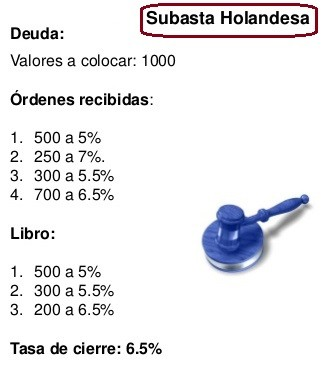
\includegraphics[scale=0.7]{Graphics/subasta-holandesa1.jpg}
      \caption{Ejemplo de subasta holandesa en el mercado de deuda}
      \label{dutch_auction}
    \end{figure}

\section{Blockchain} % \hspace*{}
  Las subastas tradicionales usualmente requieren una tercera persona, ya sea un subastador o una 
  casa de subastas que maneje el proceso completo de subasta, lo cual puede llegar a tener muy altos
  impuestos por comisiones. También sufren de un punto de fallo, los subastadores pueden en ocasiones 
  tener malas intenciones \parencite{wu2019}. En este contexto, \textit{blockchain} surge como una plataforma descentralizada que
  puede ser empleada para aplicaciones de subastas en línea confiables. En 2018, por primera vez en el 
  mundo una colección de arte valuada en varios millones de dólares perteneciente a Andy Warhol fue tokenizada
  y subastada satisfactoriamente, usando la \textit{blockchain} de Ethereum \parencite{wood2021,emem}. Es también
  conocido que una de las mayores casas de subastas (e.g., Sotheby’s and Christie’s) está activamente
  trabajando en aplicar \textit{blockchain} para subastas seguras y confiables \parencite{neuendorf2018}. 

  % On the one hand, traditional centralized auctions usually require a third-party auctioneer or auction 
  % house to manage the entire auction process, which is expensive due to high commission fees. They also 
  % suffer from a single point of failure, as auctioneers can potentially be malicious in some cases [11]. 
  % In this context, blockchain has emerged as a decentralized platform to support trustworthy online 
  % auction applications. In 2018, for the first time in the world, multi- million dollar artworks by Andy 
  % Warhol were tokenized and auctioned successfully using the Ethereum blockchain [12],[13]. It is also 
  % reported that major auction houses (e.g., Sotheby’s and Christie’s) are actively working on applying 
  % blockchain in secure and trusted auction use cases [14].

  La tecnología \textit{blockchain} elimina efectivamente los intermediarios, por lo tanto, reduce los costos de 
  transacción y asegura la confianza entre las partes interesadas en la subasta. En general, la tecnología
  \textit{blockchain} puede mejorar las subastas en los siguientes aspectos \parencite{shi2021}:
  
  - Inmutabilidad de las transacciones de la subasta. Cada transacción ejecutada en la \textit{blockchain} es pública, verificable e inmutable.
  Esto significa que la \textit{blockchain} puede ser empleada como dispositivo de certificado de auditoría que previene que los participantes
  hagan trampa durante la subasta. El ganador puede usar la \textit{blockchain} como prueba de la transacción.
  
  - Automatización del proceso de subasta. Un contrato inteligente automatiza el proceso de la subasta en la \textit{blockchain}. Casi toda 
  la lógica de la subasta puede ser predefinida en contratos inteligentes para facilitar el intercambio de bienes y servicios, así como
  el pago de los tokens.

  - Descentralización del manejo de la subasta. No hay necesidad de designar una tercera persona como subastador, que asegure la 
  confiabilidad. Las tradicionales subastas centralizadas pueden ser muy costosas y sujeta a posibles subastadores tramposos; casas
  de subastas típicamente cargan del 8 al 20\% como comisión. 

  - Flexibilidad en el pago de la subasta. Las criptomonedas existentes en la \textit{blockchain} pueden mejorar la seguridad y 
  flexibilidad del pago de la subasta. Al mismo tiempo, un sistema de pago descentralizado no necesita de intermediarios 
  financieros, haciendo
  las transacciones más convenientes y menos costosas. %page 6

  \subsection{Quorum} \hspace*{}

    \textit{Blockchain} es de los términos más usados en el mundo de la tecnología en estos días. Mientras esta tecnología es el elemento núcleo 
    de las criptomonedas que están llegando a los mercados financieros, su utilidad no es limitada a las criptos y tiene muchos más casos 
    de uso. Con el pasar de los años, diferentes plataformas \textit{blockchain} han sido desarrolladas con sus propios mecanismos de consenso
    \footnote{Por ser la blockchain un libro contable distribuido y no centralizado, se requiere establecer un mecanismo para que todos 
    los participantes en la red estén de acuerdo en el contenido sobre el contenido del libro contable. Esto es lo que se conoce 
    como un mecanismo de consenso.} y 
    métodos de encriptación.

    Una de estas plataformas es la \textit{blockchain} de Quorum, la cual ha ganado popularidad en los últimos tiempos, como resultado de 
    la larga
    lista de casos de uso que Quorum provee a sus usuarios. La red de Quorum está basada en una bifurcación\footnote{Se considera una 
    bifurcación (en inglés \textit{fork}) al desarrollo de un proyecto informático tomando como base un código fuente que ya existe e 
    iniciar un desarrollo independiente, creando así software distinto y separado.} de la \textit{blockchain} de Ethereum.
    Es un protocolo \textit{blockchain} de \href{https://github.com/ConsenSys/quorum}{código abierto} especialmente diseñado para usar en redes 
    \textit{blockchain} privadas. Algo a destacar de esta red
    es su nueva característica, llamada \textit{"private transaction identifier"}, que asegura la privacidad de los datos. El objetivo de
    construir Quorum es utilizar la tecnología existente tanto como sea posible. Por lo tanto, incluso si la red Ethereum se somete a 
    diferentes actualizaciones en el futuro, habría pocos o ningún cambio en la \textit{blockchain} de Quorum para mantener la sincronización entre
    estas redes.
    % https://www.lcx.com/a-guide-to-quorum-blockchain/

    % Quorum fue creada por el super banco JPMorgan Chase, pero en 2020 fue adquirida la plataforma por ConsenSys empresa de tecnología de
    % sofware blockchain fundada por Joseph Lubin y con sede en la ciudad de New York. Por esa razón en ocasiones se le llama a la 
    % blockchain como ConsenSys Quorum
    % https://www.coindesk.com/business/2020/08/25/consensys-acquires-jpmorgans-quorum-blockchain/

  \subsection{Subastas a ciegas sobre \textit{blockchain}}\label{section:blind_auction_protocols}
    Las subastas sobre \textit{blockchain} han sido una área centro de muchas investigaciones en los últimos años, razón por la cual ya se
    han investigado algunos protocolos de subastas a ciegas sobre \textit{blockchain}. Algunos de ellos son:    

    - Kosba et al. (\citeyear{kosba2016hawk}) propusieron Hawk, una combinación de la privacidad de 
    Zcash\footnote{Zcash es una criptomoneda que 
    utiliza criptografía aplicada avanzada para proporcionar una mayor privacidad a través de direcciones 
    protegidas. Es la primera aplicación práctica de zk-SNARK, un tipo específico de prueba de 
    conocimiento cero. \parencite{zcash}.} 
    con la programabilidad
    de Ethereum. Contratos inteligentes que preservan la privacidad fueron empleados para manejar la 
    privacidad de las transacciones en la \textit{blockchain} de Ethereum. Ellos se enfocan en presentar
    un \textit{framework} que puede simultáneamente admitir varias aplicaciones como subasta de puja sellada,
    el juego de piedra, papel y tijera, aplicación de \textit{crowdfunding}\footnote{Es un mecanismo colaborativo de financiación de 
    proyectos, desarrollado sobre la base de las nuevas tecnologías.} e intercambiar instrumentos 
    financieros. La principal limitación de Hawk es que depende de un administrador al que se le confía
    explícitamente que no filtre entradas secretas a los contratos inteligentes; dependiendo de esta manera
    de una tercera persona.

%     proposed Hawk, a combination of
% the privacy of Zcash with the programmability of Ethereum. The privacy preserving Smart
% Contracts have been employed to handle transactional privacy on Ethereum blockchain.
% They focused on presenting a framework which can simultaneously support several ap-
% plications such as sealed-bid auction, rock paper scissor game, crowdfunding application
% and swap financial instrument. The main limitation of Hawk is that it relies on a manager
% trusted explicitly not to leak secret inputs to Smart Contract.


% Hawk[KMS+ 15] focuses on protecting the privacy of transactions using zk-
% SNARKs: later works like [Solidus[CZJ+ 17], Confidential Transactions[Gib16],
% Bolt[GM16]] provide secure transactions at the protocol level with more
% 40
% efficient techniques. It only mentions secure multi-party computation as
% a tentative way to replace the trusted auction manager, rejecting it as
% impractical. \parencite{sanchez2020}

    - Blass and Kerschbaum (\citeyear{blass2017strain}) presentan Strain, un protocolo para construir una subasta de puja sellada sobre
    una \textit{blockchain}, preservando la privacidad de las ofertas contra partes maliciosas. Se utiliza un tablón
    de anuncios para publicar la oferta ganadora que es determinada comparándolas por pares. Dos 
    conocimientos de prueba cero (\textit{zero-knowledge proofs (ZKP)}) diferentes son empleadas; una 
    asegura que los 
    participantes usan sus ofertas originales, bajo compromiso, y la otra ZKP asegura que el
    subastador declare el ganador, sin ninguna manipulación. 
    Los participantes maliciosos son penalizados con la revelación de su propuesta, ya que su clave privada 
    se comparte parcialmente entre todos los participantes a través de un proceso de generación distribuida
    de claves.

    % Strain [11] presented a protocol to build a blockchain-based sealed-bid auction, preserving bid privacy 
    % against malicious parties. A bulletin board is used to publish the winning bid which is determined by 
    % comparing them by pairs. Two different ZKPs ensure that the participants used the original bids under 
    % commitment and that the auctioneer declared the winner without manipulation. The malicious participant 
    % is punished by opening their commitment as their private key is partly shared among all participants 
    % through a distributed key generation process. \parencite{sharma2021}

    - Galal and Youssef (\citeyear{galalyusef2018a}) propusieron una subasta de puja sellada en la \textit{blockchain} Ethereum con contrato 
    inteligente y pruebas de conocimiento cero (\textit{zero-knowledge proofs}). Ofertantes envían sus pujas al contrato inteligente usando
    \textit{Pedersen commitment} \parencite{pedersen1991}. Los compromisos (\texit{commitments}) son secretamente revelados al subastador vía
    un esquema \textit{Public Key Encryption (PKE)}. Después de declarar el ganador, por cada oferta 
    perdedora, el subastador tiene que
    participar en un conjunto de protocolos interactivos de compromiso-desafío-verificación para demostrar 
    que la puja ganadora es mayor que 
    las pujas perdedoras y, como consecuencia, la complejidad de la interacción depende del número de ofertantes. Luego 
    \parencite{galalyusef2018b} mejoraron este protocolo presentando un contrato inteligente con una verificablemente concisa \textit{ZKP}
    que permite una sola prueba de verificación para todo el proceso de la subasta. Similar a Zcash, ellos emplearon \textit{Multi-Party 
    Computation (MPC)}\footnote{El objetivo de los protocolos de computación multiparte (MPC) es
    permitir a un conjunto de participantes calcular el resultado
    de una función de sus entradas privadas, revelando el mínimo
    de información} entre el subastador y pujantes. El esquema propuesto implementa la validez, imparcialidad
    y secreto de las transacciones en la subasta. Sin embargo, depende de un subastador externo.
    
%     Galal and Youssef [12] presented a smart contract for verifiable first-price sealed-bid
% auction on the Ethereum blockchain. Bidders submit their bids to a smart contract using
% Pedersen commitment [13]. The commitments are secretly revealed to the auctioneer via
% a Public Key Encryption (PKE) scheme. After declaring the winner, for each losing bid,
% the auctioneer has to engage into a set of interactive commit-challenge-verify protocols
% to prove that the winning bid is greater than the losing bid and therefore, the complexity
% of interaction depends on the number of bidders. Later, Galal and Youssef [3] improved
% this protocol and presented a Smart Contract with succinctly verifiable ZKP which enables
% single proof verification for the whole auction process. Similar to Zcash, they used MPC
% among auctioneer and bidders to derive Common Reference String (CRS) during Zero-
% Knowledge Succinct Non-interactive ARgument of Knowledge (zk-SNARK) set up. \parencite{sharma2021}
    
    % The proposed scheme
    % implements the validity, fairness, secrecy of the auction
    % transaction. However, the proposed scheme depended on the
    % third-party auctioneer \parencite{li2021}

    - Sánchez (\citeyear{sanchez2020}) propone un contrato inteligente privado y verificable, se introduce 
    como una combinación de \textit{Multi-Party 
    Computation} segura y \textit{Proof-carrying code}\footnote{Es un mecanismo de software que permite que 
    un sistema host verifique las 
    propiedades de una aplicación a través de una prueba formal que acompaña al código ejecutable de la 
    aplicación.} enfocada 
    principalmente en garantizar la correctitud, privacidad y 
    verificabilidad para contratos inteligentes en la \textit{blockchain}. Este enfoque puede ser utilizado 
    para varios tipos de aplicaciones tales
    como \textit{crowdfundings} privados y verificables, fondos de inversión y subastas dobles para 
    intercambios descentralizados.

%     A
% private and verifiable smart contract approach [10], introduced as a combination of secure
% MPC and proof-carrying code focusing primarily on correctness, privacy and verifiability
% guarantees for smart contracts on blockchains. The approach is well applicable to several
% applications such as private and verifiable crowdfundings, investment funds and double
% auctions for decentralized exchanges.

    - Sharma et al. (\citeyear{sharma2021}) introdujeron un protocolo genérico para comercio anónimo de 
    manera justa usando solamente construcción estándar de bloques criptográficos. Las propiedades confidencialidad y anonimato son alcanzadas utilizando 
    \textit{Designated Verifier Ring
    Signature (DVRS)} y la transparencia y auditabilidad de la plataforma \textit{blockchain} se aprovecha 
    para realizar el proceso de subasta
    públicamente verificable. Asume la existencia de una \textit{blockchain} que permita transacciones 
    anónimas y confidenciales.
    También analiza la eficiencia de emplear primitivas criptográficas en la \textit{blockchain} de 
    Ethereum e investigar la complejidad
    y vulnerabilidades que un entorno \textit{blockchain} podría introducir durante la implementación.

%     We have introduced a generic protocol for anonymous fair trade using only standard cryptographic building blocks. The confidentiality and anonymity properties are achieved
% using DVRS and the transparency and auditability of blockchain platforms is leveraged in
% order to make the auction process publicly verifiable. In this paper, we assume the existence
% of a blockchain facilitating anonymous and confidential transactions. We also analyzed the
% efficiency of using such cryptographic primitives on Ethereum blockchain and investigate
% the complexity and vulnerabilities that a blockchain environment might introduce during
% implementation.

    - Li and Xue (\citeyear{li2021}) proponen un esquema de subasta electrónica de puja sellada basada en \textit{blockchain} con algoritmo de 
    compromiso, contratos inteligentes y \textit{zero-knowledge proof (ZKP)} para proteger la fuga de información de las pujas y verificar
    el resultado de la subasta con todos los ofertantes anónimamente, que implementa satisfactoriamente la seguridad y justicia de la 
    subasta sin necesidad de un subastador externo. El esquema sugerido presenta limitaciones en cuanto al 
    tiempo de corrida. El tiempo 
    de ejecución de dos de las fases, la fase abierta y fase final, está determinado por el número de 
    ofertantes. Esto significa que 
    la subasta se convertiría en un trabajo que consume mucho tiempo en el caso de ser usado en 
    plataformas abiertas como Internet.

%     In this paper, we proposed a sealed-bid e-auction scheme
% based on blockchains with commitment algorithm, smart
% contracts, and zero-knowledge proof to protect the bid
% information from leakage and verify the auction result with
% all bidders anonymously, which successfully implemented
% the secure and fair auction without the third-party
% auctioneer.

%     It should be noted that the proposed scheme has limi-
% tations in running performance. As was discussed in Section
% 5.1, the execution time of the open phase and finish phase
% was determined by the number of bidders. It means that the
% auction would become a time-consuming work if conducted
% in the open platforms such as Internet.

% -----------------------------------------------------------------------------------------

    De acuerdo a la revisión de la literatura hecha anteriormente, los estudios relacionados tienen algunos defectos para los 
    esquemas de subasta de puja sellada. En opinión del autor de esta investigación, tales dificultades serían:

    1 - Riesgo del modo de transacción centralizado: como se discutió anteriormente, en subastas 
    tradicionales todas las transacciones
    están en control de los subastadores. Ha sido demostrado que subastadores no confiables pueden causar filtración del precio de la puja
    y alterar el resultado de la subasta. En los estudios relacionados, la mayoría de subastas electrónicas, incluso las basadas en 
    \textit{blockchain}, todavía utilizan subastadores para controlar las transacciones. Por lo tanto, la equidad y fiabilidad de las 
    subastas no están perfectamente garantizadas.

    2 - Ocultación de precios incompleta: ocultar el precio de las pujas es el núcleo de las subastas de puja sellada. En la mayoría de los estudios 
    relacionados, el precio de la puja es protegido por encriptación. Sin embargo, en la fase abierta, el precio de la puja es desencriptado
    y directamente revelado por verificación, lo cual puede causar filtración de precios.

%     According to the above literature review, the related
% studies still have some defects in sealed-bid auction schemes.
% (1) The risks from centralized transaction mode: as was
% discussed above, in traditional auctions, the whole trans-
% actions are in the control of auctioneers. It has been proved
% that the untrusted auctioneers may cause the bid price
% leakage and tamper with the auction results. In related
% studies, most e-auction schemes, even those based on
% blockchains, still took auctioneers as the transaction con-
% trollers. Therefore, the fairness and reliability of auctions
% were not perfectly guaranteed. 
% (2) Incomplete price hiding:
% price hiding is the core of sealed-bid auctions. In most
% related studies, the bid price is protected by encryption.
% However, in the open phase, the bid price is decrypted and
% directly revealed for verification, which may cause price
% leakage and the benefits damage of the winning bidder.
